% D.16 矩形 ABCD，AB=6，BC=8；P∈BC，PE⊥AC，PF⊥BD
\documentclass[tikz,border=4pt]{standalone}
\usepackage{ctex}
\usepackage{amsmath}
\usetikzlibrary{calc}
\begin{document}
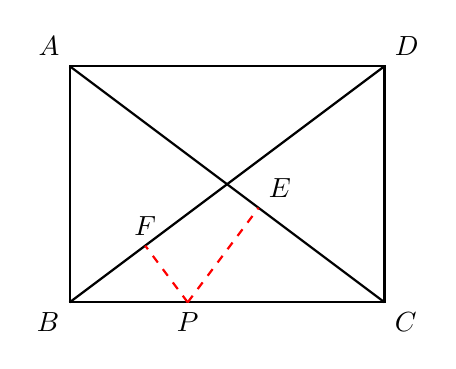
\begin{tikzpicture}[scale=0.5, thick]
  \coordinate (A) at (0, 6);
  \coordinate (B) at (0, 0);
  \coordinate (C) at (8, 0);
  \coordinate (D) at (8, 6);
  \coordinate (P) at (3, 0);
  % E = P 在 AC 上的投影；AC: A->C 方向 (8,-6)，|AC|=10
  \pgfmathsetmacro{\tE}{((3-0)*8 + (0-6)*(-6))/(8*8+6*6)}
  \coordinate (E) at ({0 + \tE*8}, {6 + \tE*(-6)});
  % F = P 在 BD 上的投影；BD: B(0,0)->D(8,6)
  \pgfmathsetmacro{\tF}{(3*8 + 0*6)/(8*8+6*6)}
  \coordinate (F) at ({\tF*8}, {\tF*6});

  \draw (A) -- (B) -- (C) -- (D) -- cycle;
  \draw (A) -- (C);
  \draw (B) -- (D);
  \draw[red, dashed] (P) -- (E);
  \draw[red, dashed] (P) -- (F);

  \node[above left]  at (A) {$A$};
  \node[below left]  at (B) {$B$};
  \node[below right] at (C) {$C$};
  \node[above right] at (D) {$D$};
  \node[below]       at (P) {$P$};
  \node[above right] at (E) {$E$};
  \node[above]       at (F) {$F$};
\end{tikzpicture}
\end{document}
